\documentclass{standalone}

\usepackage{ifthen}
\usepackage{tikz}
\usetikzlibrary{shapes, positioning, arrows.meta}

\begin{document}

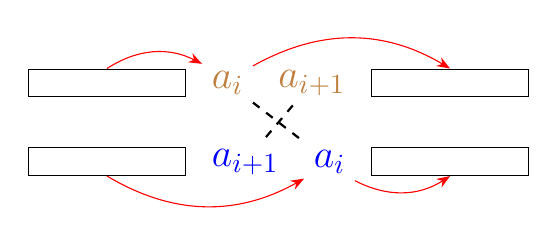
\begin{tikzpicture}[swap/.style = {dashed, thick},
	inv/.style = {>=Stealth, ->, red},
	ele/.style = {font = \Large},
  seq/.style = {rectangle, minimum width = 2cm, inner sep = 5pt, draw},]

  \node (pre) [seq] {};
  \node (ai) [ele, right = 0.20cm of pre, brown] {$a_{i}$};
  \node (ai1) [ele, right = 0.20cm of ai, brown] {$a_{i+1}$};
  \node (post) [seq, right = 0.20cm of ai1] {};

  \begin{scope}[yshift = -1cm]
	\node (spre) [seq] {};
	\node (sai1) [ele, right = 0.20cm of spre, blue] {$a_{i+1}$};
	\node (sai) [ele, right = 0.20cm of sai1, blue] {$a_{i}$};
	\node (spost) [seq, right = 0.20cm of sai] {};
  \end{scope}
  
  \draw [swap] (ai) to (sai);
  \draw [swap] (ai1) to (sai1);

  \draw [inv, bend left] (pre.north) to (ai);
  \draw [inv, bend right] (spre.south) to (sai);

  \draw [inv, bend left] (ai) to (post.north);
  \draw [inv, bend right] (sai) to (spost.south);
\end{tikzpicture}
\end{document}
